% !TEX root = ../main.tex
\section{Approach}
\label{sec:approach}
This section describes a method for accurately estimating poses for square fiducial tags in noisy settings by fusing RGBD data. The process of detecting and decoding the tag is identical to previous fiducial tag systems. After the tag corners are detected, they are treated as approximated locations of the true corners. Using the corners, the method implicitly evaluate the depth data and RGB data as two separate observations and fuse them to minimize the error in 2D and 3D space.

There are three distinct components to this method. First, we find the plane in $SO(3)$ containing the tag using depth data and detected corners. Secondly, an approximate initial pose is computed using the depth plane. Finally, the method refines the initial pose using the RGB data by minimizing the reprojection error within a constrained space. Each component is described in detail in the following subsections. 

\subsection{Depth Plane Fitting}
The first step is to extract the plane which the tag is laying on. We assume that the RGBD sensor is calibrated such that depth and RGB streams are registered to the same frame. The rectangular patch of points in the depth image bounded by the approximated corner pixels $\boldsymbol{y} = [y_1, y_2, y_3, y_4]$ contains the range information of all the points on the tag. Here we take advantage of the planar characteristic of the tag. By fitting a plane over the range data, we can constrain the pose of the tag to be on the plane.

The raw range data retrieved from the depth sensors are generally noisy. The borders and dark regions of the tag produce unreliable range data and artifacts due to a weakness of our depth sensor (time of flight sensor from Kinect V2). Therefore, we first filter the data by removing points too far from the median before fitting the plane. Nevertheless, the remaining points could have a large variance depending on the lighting condition and the magnitude of the in-plane rotation. The accuracy of the plane fit and initial pose estimation is directly affected by the noise level of data. We will characterize the uncertainty of the plane fit and adjust the weight of the depth pose estimation accordingly during the fusing stage.

In implementation, we used a Bayesian plane fitting algorithm described in~\citep{pathak2010uncertainty} which computes the Hessian Normal parameters $[\boldsymbol{\hat{n}}, d]$ of a plane for noisy range data through optimizing
\begin{IEEEeqnarray}{c}
\min _{\boldsymbol{\hat{n}}, d} \sum_{j=1}^{N} 
	\frac{(p_j(\boldsymbol{\hat{n}} \cdot \boldsymbol{\hat{m}_j}) -d)^2}
		 {(\boldsymbol{\hat{n}} \cdot \boldsymbol{\hat{m}_j})^2\sigma ^2\{\bar{p}_j \} }
\label{eq:gaussian_noise}
\end{IEEEeqnarray}
where $\boldsymbol{\hat{n}}$ is the local normal to the planar surface of the depth point and $\boldsymbol{\hat{m_j}}$ is the measurement direction for the sensor for point $p_j$. 
The algorithm in the paper assumes a radial Gaussian noise in the range data $p_j$ with the standard deviation modeled by a function in the form
\begin{IEEEeqnarray}{c}
\sigma \{ \bar{p_j} \} = \frac{kd^2}{ \| \boldsymbol{\hat{n}} \cdot \boldsymbol{\hat{m}_j} \| } 
\IEEEeqnarraynumspace
\label{eq:gaussian_noise}
\end{IEEEeqnarray}
The coefficient $k > 0$ is an estimated value obtained from sensor calibration. In our implementation, we obtained $k$ by using the Kinect V2 model obtained from \citep{nguyen2012modeling}. 

An important result we used from \citep{pathak2010uncertainty} is the covariance matrix for the plane-parameters. The covariance is obtained by taking the \textit{Moore-Penrose generalized inverse} of Hessian matrix computed from the Lagrangian. It characterizes the uncertainty of the plane fit and implicitly measures the relative accuracy of the depth data.

\begin{figure}
\centering
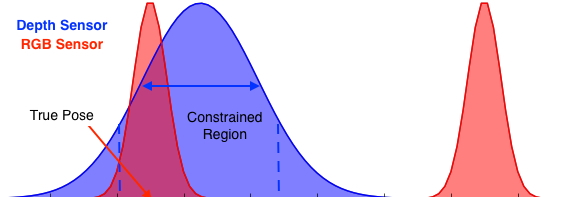
\includegraphics[width=\columnwidth]{figs/optimization_visualization_fig}
\caption{An abstract visualization of the optimization constraints. The blue curve is the initial pose estimation obtained from the depth plane. The red curves are the ambiguous poses from the RGB image. We constrained the region of optimization based on how well we fit the depth plane.}
\label{fig:optimization}
\end{figure}

\subsection{Initial Pose Estimation}
The 6 DOF pose of the tag can be described as the transformation $[R, \boldsymbol{t}]$ aligning the tag frame's coordinate system and the sensory frame's coordinate system of the robot. The depth plane $D [ \boldsymbol{\hat{n}}, d]$ alone is insufficient to determine the transformation as it only defines 3 DOF. Since the depth plane was computed base on the approximate center of the tag, we can use the center of the tag and center of the plane as a pair point correspondence. However, there are still infinite number of valid poses rotating about the normal $\boldsymbol{\hat{n}}$. One solution is to constrain the pose by using a corner as an extra point correspondence to solve for the optimal rotation. In practice, the accuracy of this method largely depends on the depth accuracy of the chosen corner point. 


\begin{figure}
\subfloat[RGB]{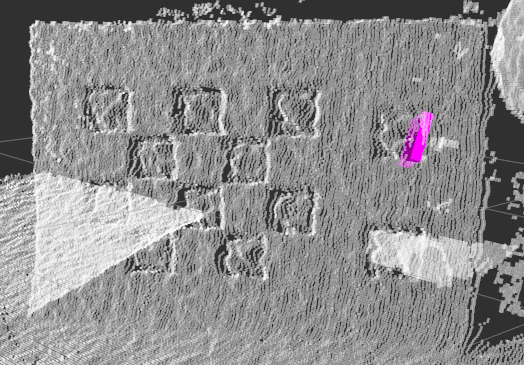
\includegraphics[width=125px, height=88px]{figs/rgb_result}}
\subfloat[RGBD]{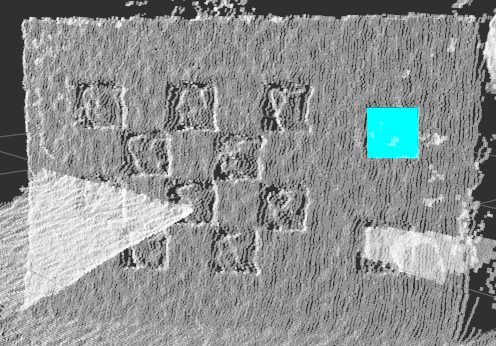
\includegraphics[width=125px, height=88px]{figs/rgbd_result}}
\caption{The pose of the Apriltag visualized in RViz computed using the original library VS our RGBD fused method.}
\label{fig:result_compare}
\end{figure}

\begin{figure*}[h]
\subfloat[RGB image at 60$^{\circ}$]{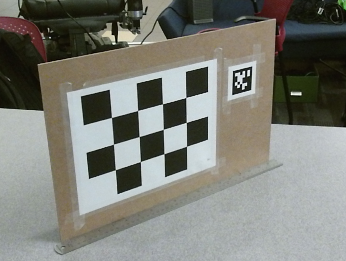
\includegraphics[width=\columnwidth, height=160px]{figs/result_figs/rgb_smallfig}
\label{fig:exp_setup}}
\subfloat[Rotation errors across 1000 trials]{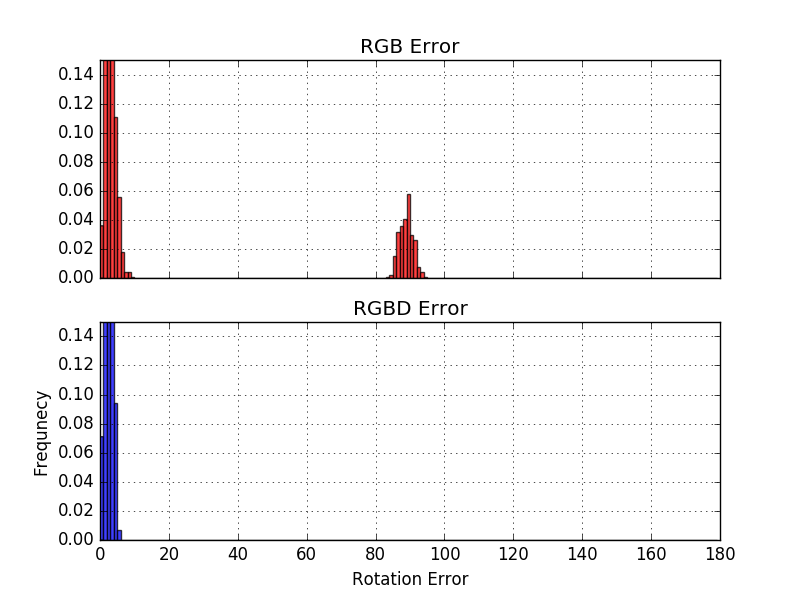
\includegraphics[width=\columnwidth, height=170px]{figs/result_figs/result_0005}
\label{fig:bimodal}} \\
\caption{An example of the experimental setup in \ref{fig:exp_setup}. Groundtruth is computed from a large chessboard where the relative transformation to the tag is known. Each data collection, shown in \ref{fig:bimodal}, is ran through $1000$ trails and pose errors are measured.}
\label{fig:angle_result}
\end{figure*}

An alternative is to use all 4 detected corners as 4 pairs of point correspondences for the optimization. We projected the detected corners onto $D [ \boldsymbol{\hat{n}}, d]$ to get the coordinates $\boldsymbol{p} = [p_1, p_2, p_3, p_4]$ in the robot sensory frame. The corner coordinates $\boldsymbol{q} = [q_1, q_2, q_3, q_4]$ in the tag frame can be easily calculated since the tag is a square plane. We define the center of the tag as the origin, and the coordinates are simply the location of the corners on a Cartesian plane. Given these two sets of 3D point correspondences, the pose can be computed as a rigid body transformation estimation. Solving for the optimal transformation $[R, \boldsymbol{t}]$ requires minimizing a least squares error objective function given by:
\begin{IEEEeqnarray}{c}
[R, \boldsymbol{t}] = \argmin _{R \in SO(3), \boldsymbol{t}\in \mathbb{R}^3} \sum_{i=1}^{n} w_i \| R \boldsymbol{q_i} + \boldsymbol{t} - \boldsymbol{p_i}\| ^2
\IEEEeqnarraynumspace
\label{eq:rigid_body}
\end{IEEEeqnarray}
There are numerous approaches to solve Eq. \ref{eq:rigid_body} described in~\citep{eggert1997estimating}. Since we have very few correspondences and they are assumed to be correct, it can be computed efficiently using SVD:
\begin{IEEEeqnarray}{rCl}
& \bar{p} = \frac{1}{N} \sum_{i=1}^{N} p_i \qquad p_{ci} = p_i - \bar{p} \\
& \bar{q} = \frac{1}{N} \sum_{i=1}^{N} q_i \qquad q_{ci} = q_i - \bar{q} 
\end{IEEEeqnarray}
\begin{IEEEeqnarray}{rCl}
p_{c}^{\top}q_c &= U\Sigma V^\top \\
R & = VU^\top\\
\boldsymbol{t} & = \bar{q} - R\bar{p}
\end{IEEEeqnarray}
Here, $R$ and $\boldsymbol{t}$ are the corresponding rotation and translation components of the the transformation. The above approach minimizes the least square error of the transformation and it is robust to small errors in the correspondences. The resulting pose obtained from the range data, although not accurate, provide a good approximation for the true pose. 

\subsection{Pose Refinement}

Lastly, the pose is refined by minimizing the reprojection error in  Eq.\ref{eq:reprojection} using the initial pose estimated from the previous step. The camera is assumed to be calibrated and the camera projection model $K$ is known. Here, $R^*$ and $\boldsymbol{t^{*}}$ are the optimal pose in the constrained optimization function
\begin{IEEEeqnarray*}{rCl}
[R^*, \boldsymbol{t^{*}}] & = & \argmin _{R^*, \boldsymbol{t^{*}}} \sum_i^n \| (K [R^* | \boldsymbol{t^{*}}]) \boldsymbol{p_i} - \boldsymbol{y_i}\| ^2 \IEEEyesnumber \\
\label{eq:reprojection}
R^* & = & R (\Delta R) \IEEEyesnumber \\ 
\boldsymbol{t^{*}} & = & \boldsymbol{t} + R (\Delta \boldsymbol{t}) \IEEEyesnumber \\
\noindent \text{subject to:} \\ 
\Delta R & < & \Gamma_R , \; \Delta \boldsymbol{t}  <  \Gamma_t \IEEEyesnumber \\
\label{eq:refinement}
\end{IEEEeqnarray*}

Intuitively, the most optimal pose is the one with minimal reprojection error in the RGB space and align with the plane in the depth space. Therefore, the goal of the optimization is to find the local minimum closest to the initial estimation within allowable region $\Gamma$ as illustrated with Figure \ref{fig:optimization}. The key challenge is to determine the constrained region $\Gamma_R$ and $\Gamma_t$ such that it include a locally optimal pose and exclude the ambiguous pose. In most cases where the depth plane yields a good fit, this region should be small because the optimal pose is close to the initial estimate. When the depth sensor is noisy, the $\Gamma$ increases since the initial estimate might be far off. Thus, the constrained region $\Gamma$ is defined by the uncertainty in the initial estimate and it is characterized by the covariance of the plane parameters. In implementation, we used a trust-region optimization algorithm to bound the constraints. The scaling parameters for the covariance is empirically tested to obtain the best results for our robot. 


\begin{figure}
\centering
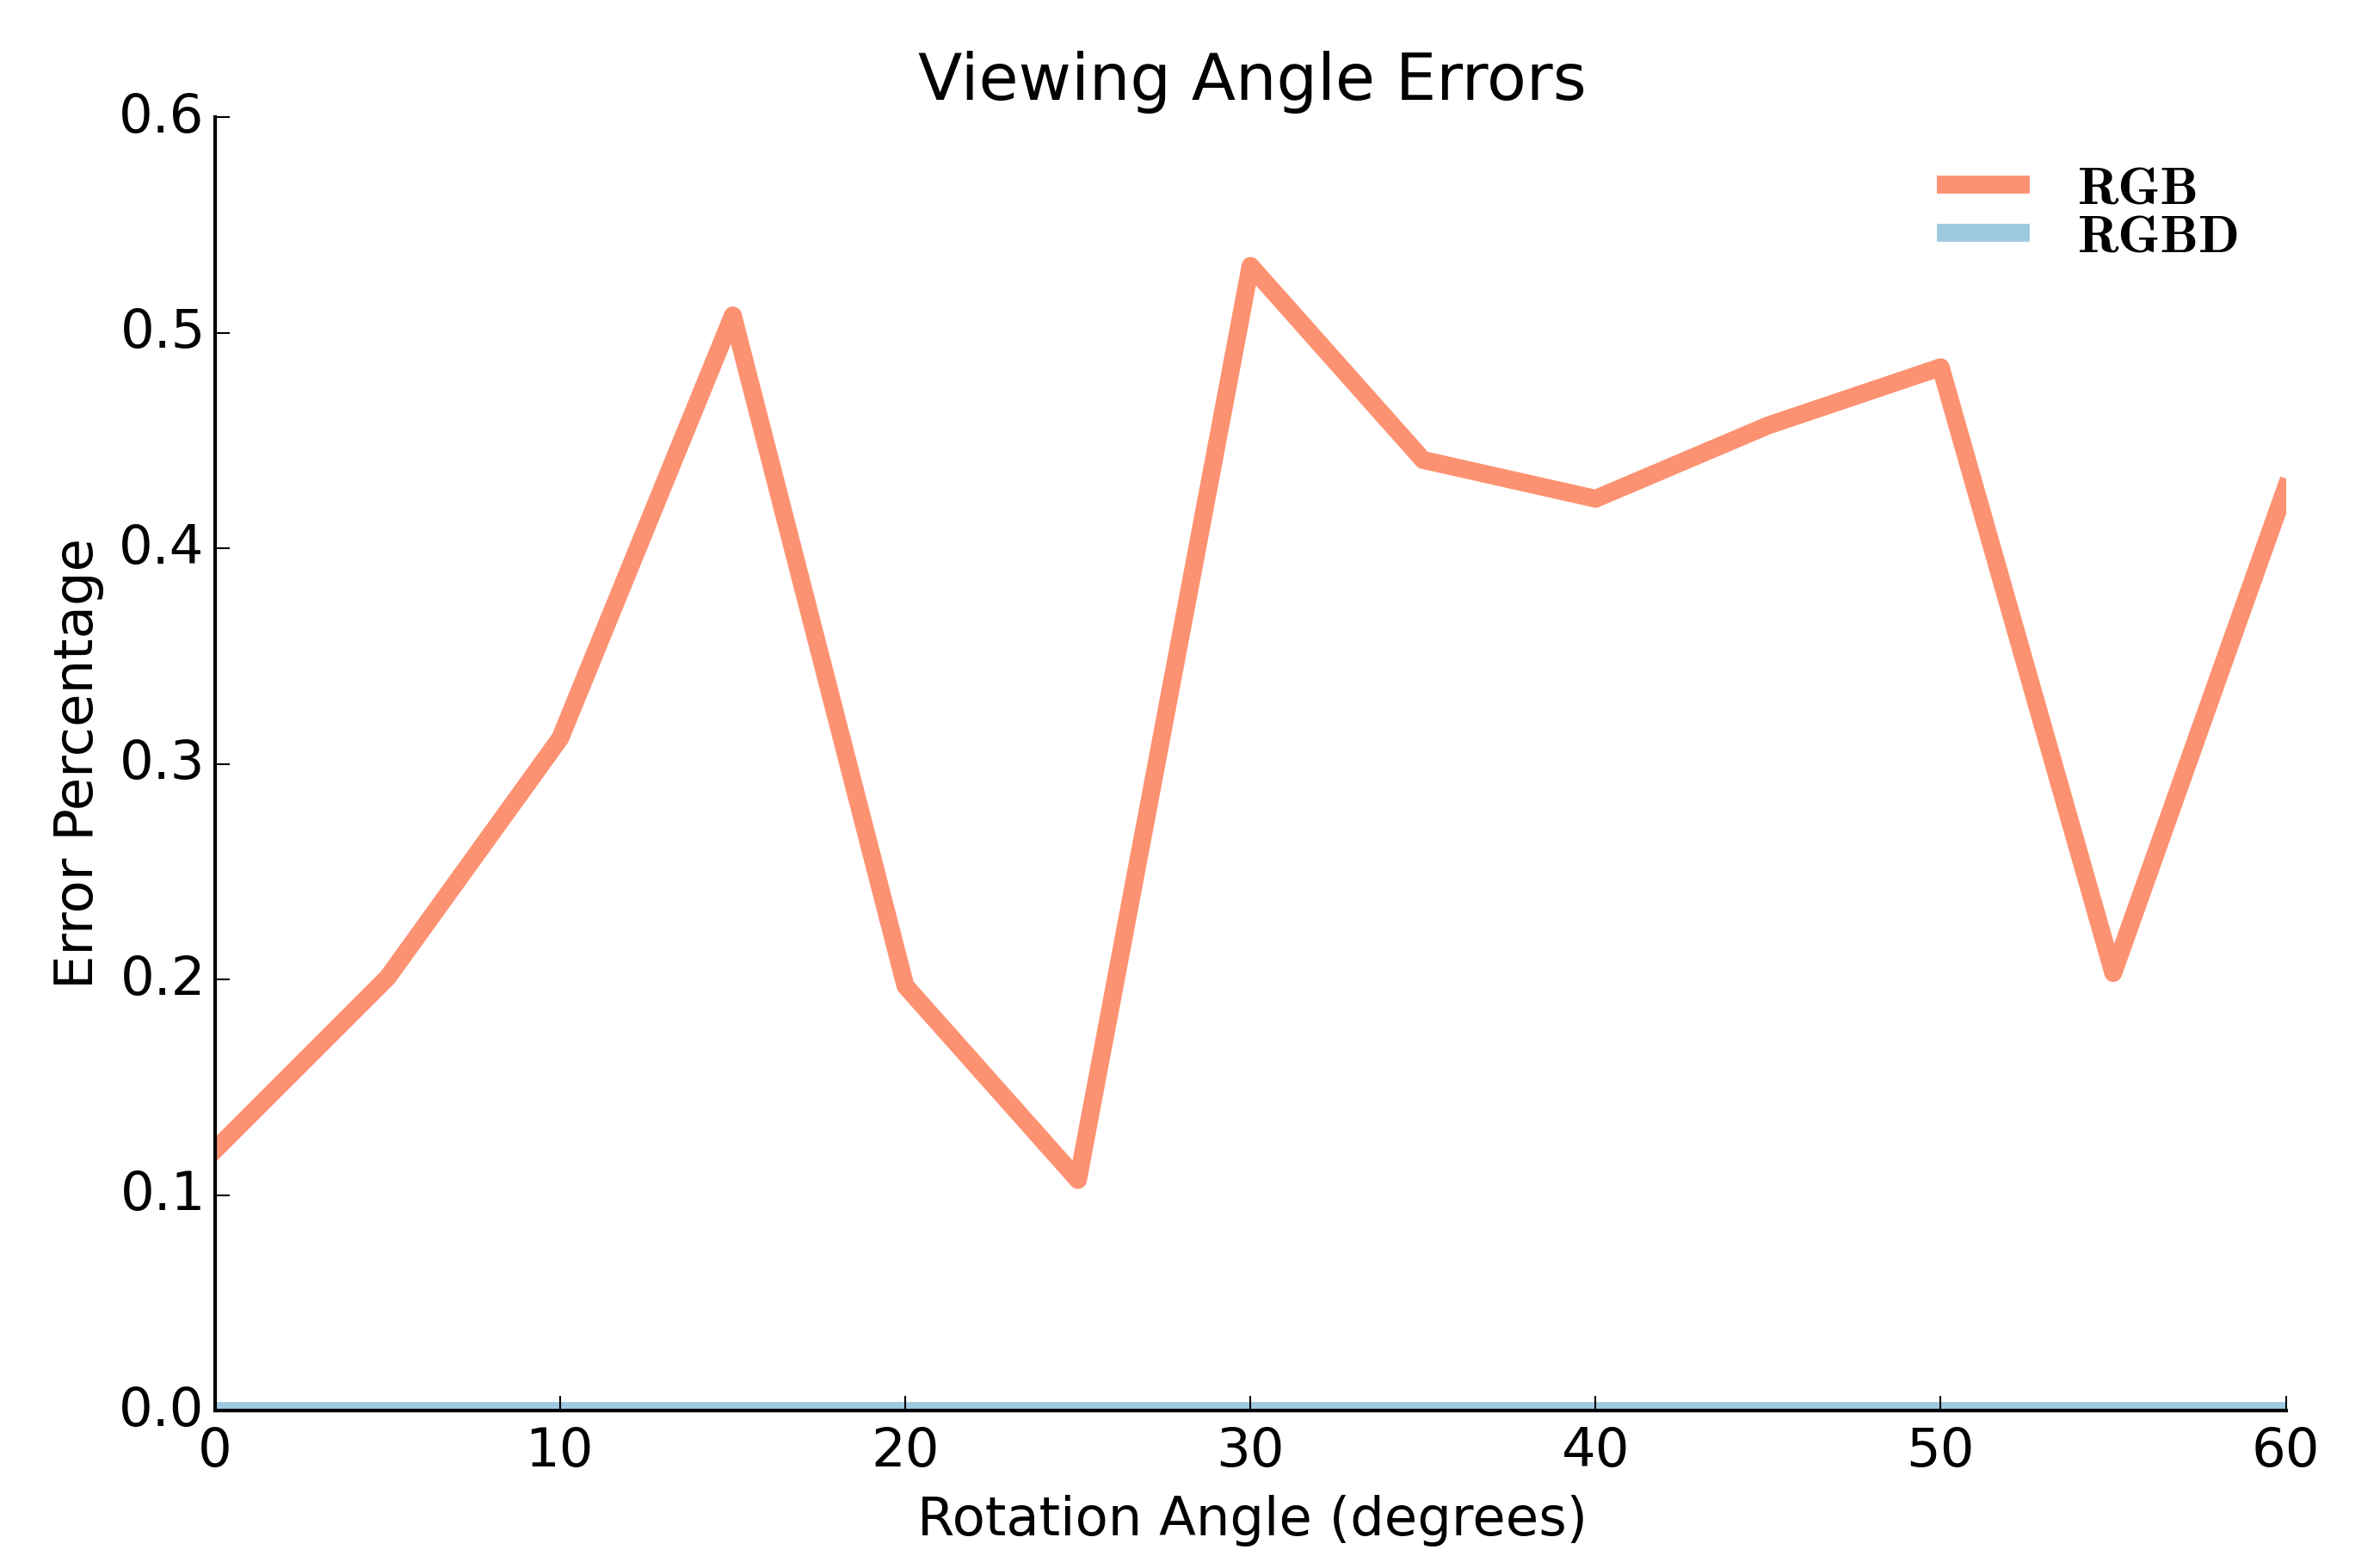
\includegraphics[width=220px, height=130px]{figs/viewing_angle_fig2}
\caption{Viewing Angle vs Error Percentage under different simulated noise level. The new RGBD based algorithm can resist noise in the RGB image and it vastly outperforms the original algorithm.}
\label{fig:viewing_result}
\end{figure}

The strength of this method is that it harness the benefits of RGB and depth information without explicitly assuming their relative accuracy. One advantage of RGBD sensors is that the camera and the depth sensor often work optimally with different constraints. In the example of Kinect, the RGB camera is sensitive to lighting and works poorly in scenes with low illumination. However, the time of flight depth sensor are unaffected by such a problem. On the hand, the time of flight sensor yield poor range results on surface edges, but the RGB camera works exceptionally well with edges where there is a high color contrast. 